%! TEX root = master.tex
\lecture{2}{Week: 1}{Continue Introduction C}

\subsubsection{Example Code}
Header files are external linked files. Ever program has to have \code{main} function which takes several command line options. The number of arguments if given by \code{argc} (argument count) and the arguments themselves via \code{argv} (argument vector)

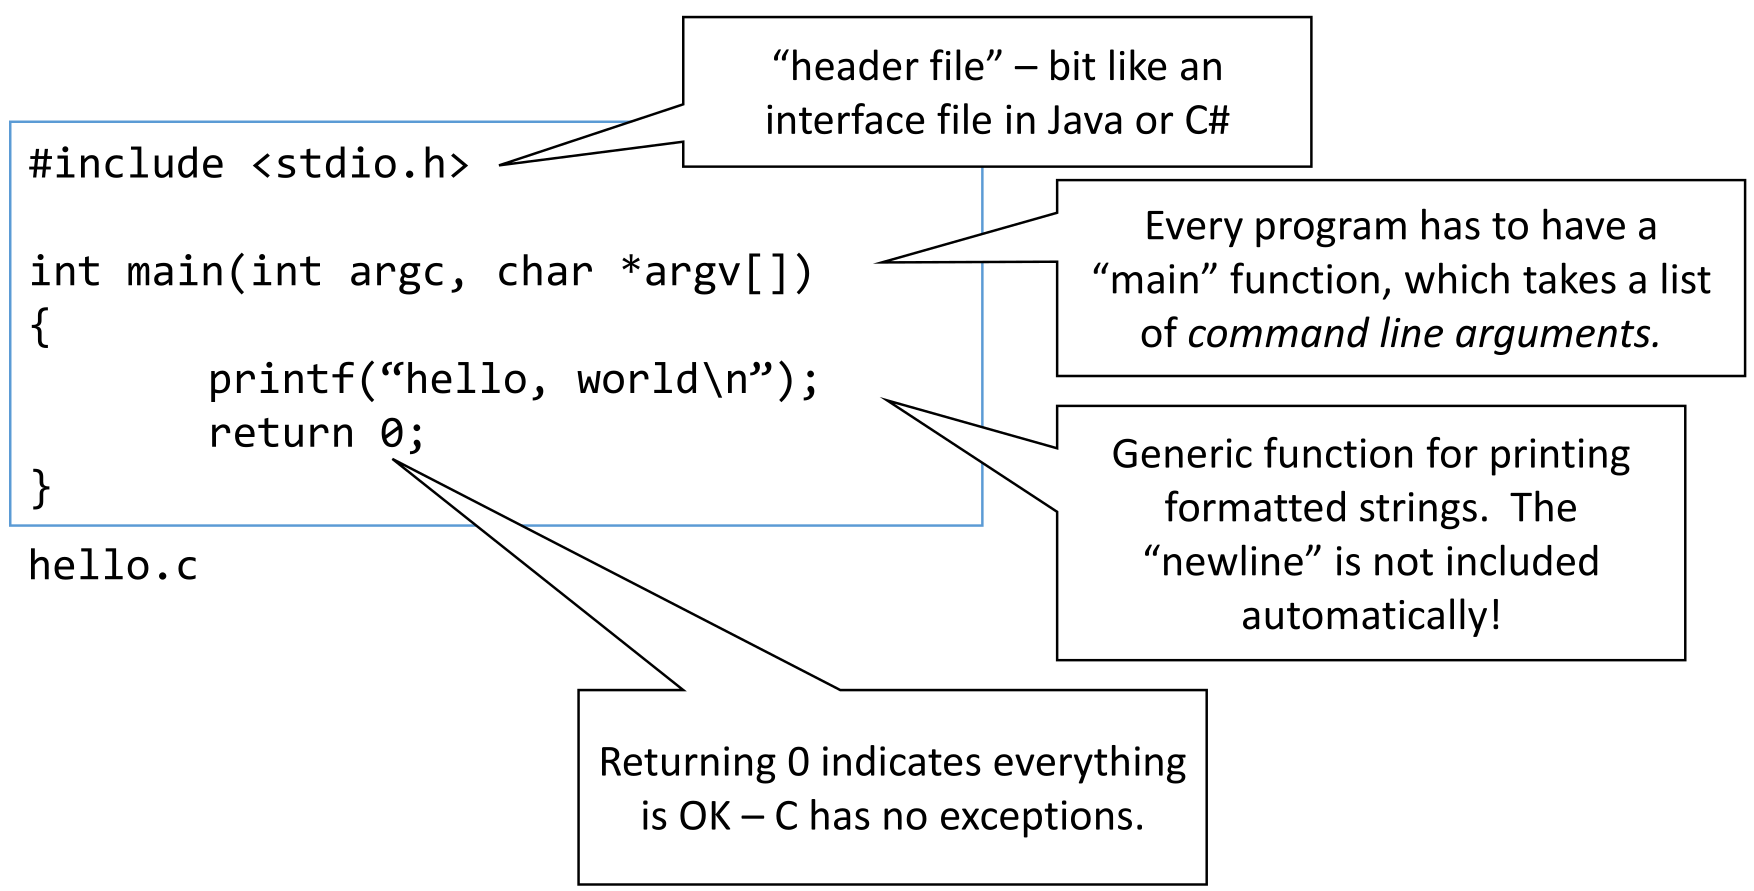
\includegraphics[width=0.8\textwidth]{02_exCode.png}

\subsubsection{Workflow}
Programmers write source code \code{.c} files and header files \code{.h}. At first, macros get substituted. Each of these files is compiled into assembly \code{.s} and then into object files \code{.o}. Object files are linked with their external libraries \code{.a} and we get an executable file. There are also libraries (shared libraries) \code{.so} which are dynamically linked while running the code.

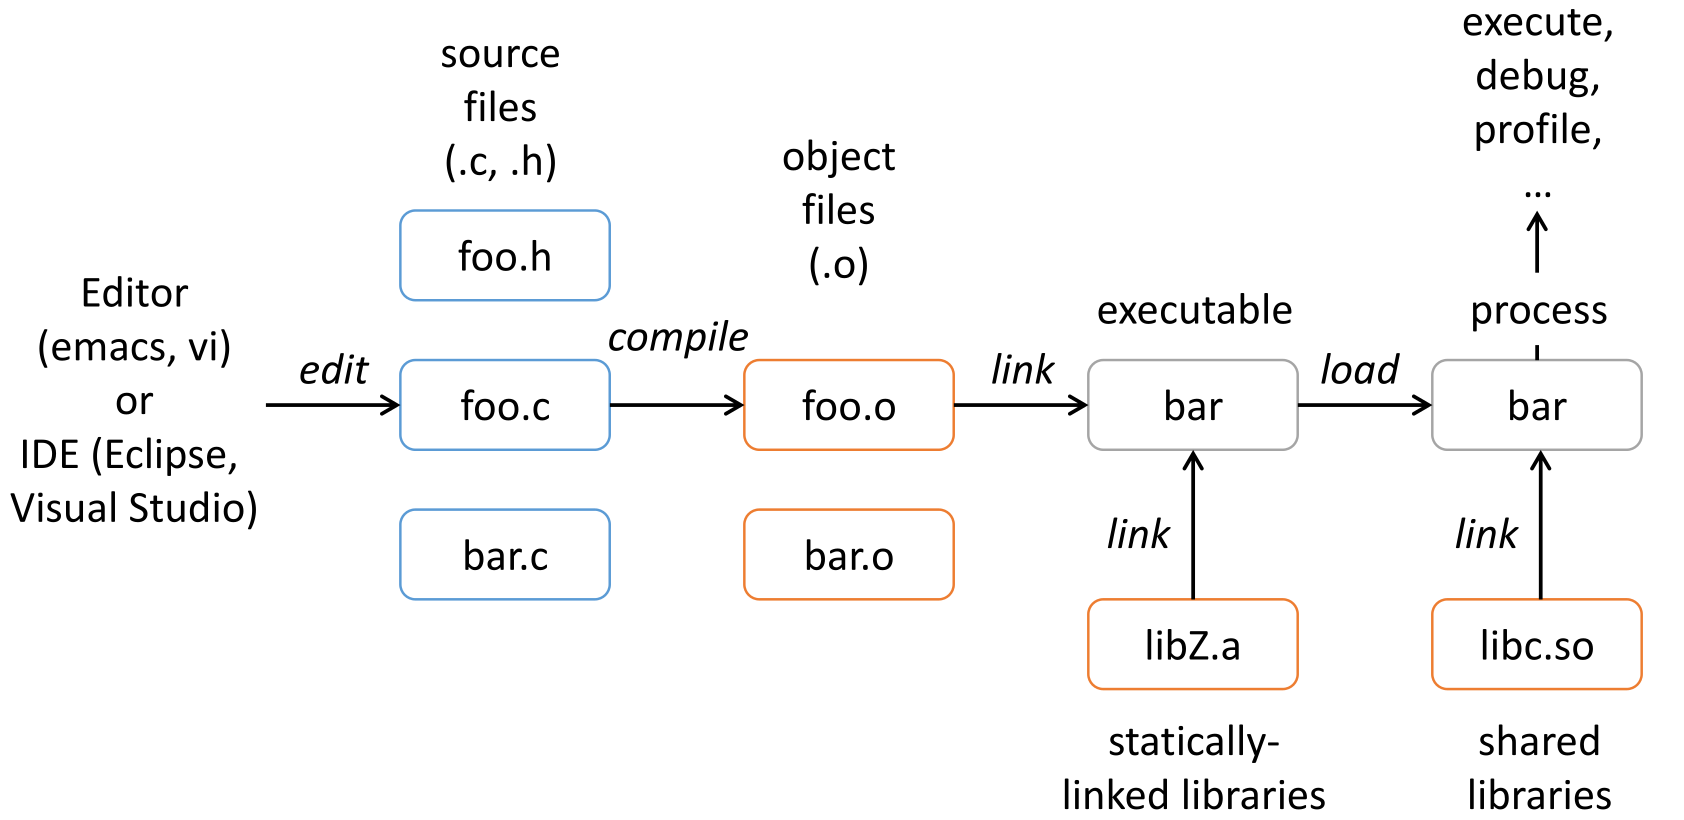
\includegraphics[width=0.8\textwidth]{02_workflow.png}

\code{gcc} is the \textit{compiler} (it does also all other parts of the workflow) we use in all exercises in this lecture.

We can stop the compilation at each stage:

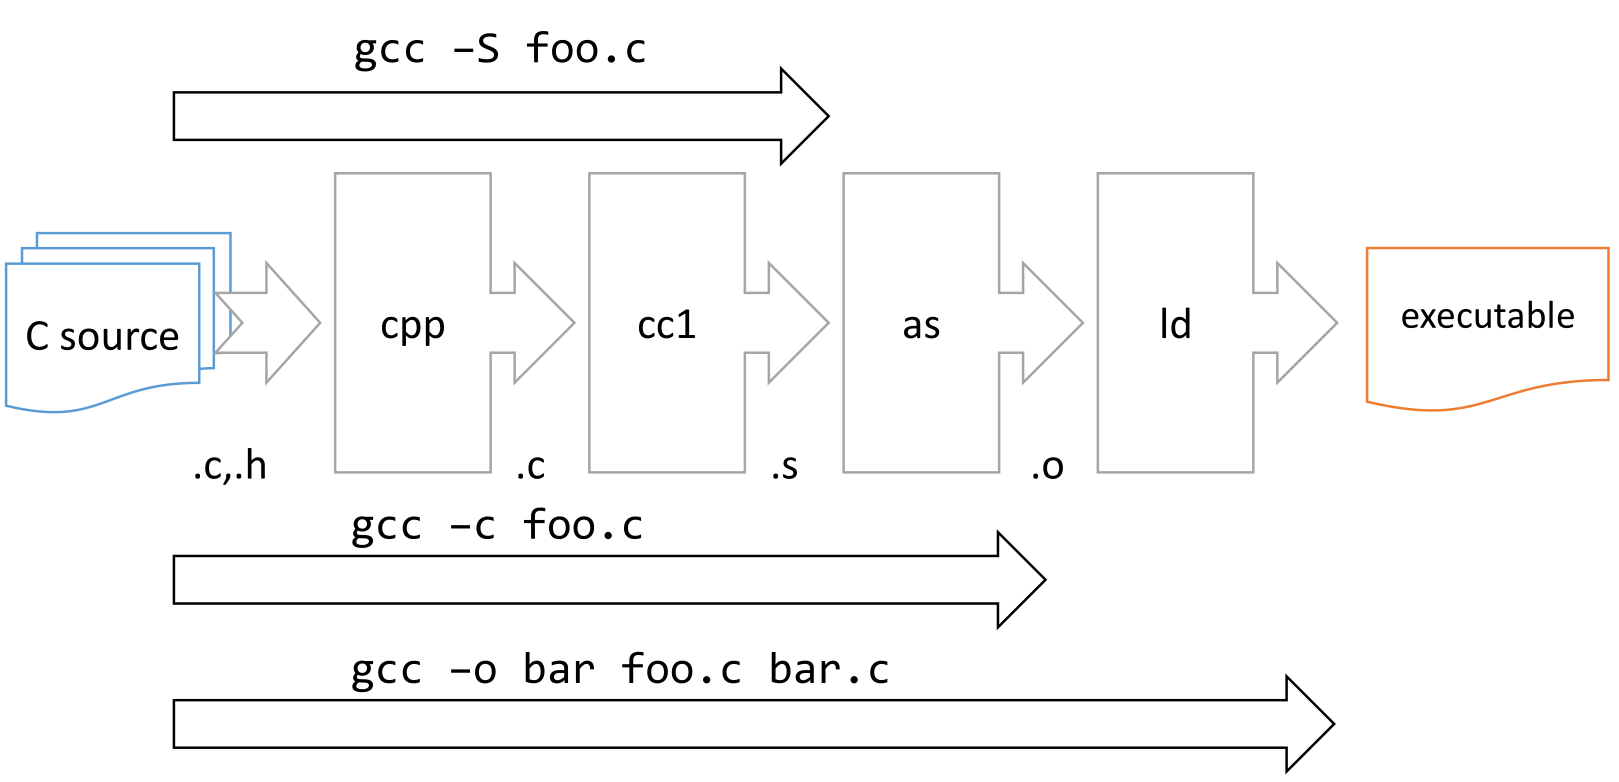
\includegraphics[width=0.8\textwidth]{02_gcc.png}

\subsection*{Control Flow}

\subsubsection{Conditionals}
They are written pretty much are we are used to.

\paragraph{If}
\begin{lstlisting}
if (Expression) {
    Statement_when_true
} else {
    Statement_when_false
}
\end{lstlisting}

The brackets can be omitted when the statements are just one line.
\begin{lstlisting}
if (Expression) Statement_when_true
else Statement_when_false
\end{lstlisting}

\paragraph{Switch}
If we not not break on a successful condition, multiple conditions may be executed.
\begin{lstlisting}
switch (Expression) {
        case Constant_1: Statement; break;
        case Constant_2: Statement; break;
        ...
        default: Statement; break;
}
\end{lstlisting}

\subsubsection{Loops}
The syntax of the three loop types available in C are as we are used to from other languages. 

If the statement is just one line, they may we written as:
\begin{itemize}
    \item \code{for (Initial; Test; Increment) Statement}
    \item \code{while (Expression) Statement}
    \item \code{do Statement while (Expression)}
\end{itemize}

\subsubsection{Other Statements}

\paragraph{Break}
Is used to break out of the current loop/switch. Unlike in Java, we cannot give a label.

\paragraph{Continue}
Stops current iteration of loop. Unlike in Java, we cannot give a label.

\paragraph{Goto}
\code{goto Label} jumps straight to \code{label}. It is controversial, but occasionally very useful. It makes code hard to read.

\subsubsection{Functions}
Functions are very similar to Java. They have a name, return type, argument types and a body.

\code{type name(paraType paraName) {body}}

The entry point to each C program is the \code{int main(int argc, char *argv[]) {body; return 0}} function. \code{argc} is the number of parameter and \code{*argv} a list of string parameter.

\code{return (Expression)} is used to return a value (may be computed by an expression) of a valid type (must conform to the defined return type).

\subsubsection{I/O}
\code{printf()} is used for outputs. The general format is that the first argument is the format string, containing special *replacement delimiters*, followed by the values to be inserted into the string. The number as well as the type of the variables must match the one in the format string.

\code{man 3 printf} for docs. 

\subsection*{Types}

\paragraph{Declarations}
Similarly as in Java, before a variable can be used, it must be declared \code{type name;}. Declaration and assignment can be combined into a single statement \code{type name = value;}.

\subparagraph{Scope}
Variables declared inside a block have a scope of only this block. Variables which are not defined inside a block have a scope of the entire program. 

\subparagraph{Static}
\code{static} in C is very different than in Java. Its meaning depends on its scope (/if it is inside/outside a block). If inside a block, the value of this variable persists between function calls. If static is used in a variable declared outside any block, the static makes that this variables is only accessible to this file (compilation unit) instead of the entire program.

\subsubsection{Types and Sizes}
\begin{table}[H]
    \centering
    \begin{tabular}{c c}
        C data type & Intel x86-64\\
        \hline
        char & 1\\
        short & 2\\
        int & 4\\
        long & 8\\
        float & 4\\
        double & 8\\
        long double & 10/16\\
    \end{tabular}
\end{table}

\subsubsection{Numbers}
Integers are signed by default. To make it more explicit, \code{signed} or \code{unsigned} can be prepended.

In standard, \code{int} have a size of $4$ bytes. Sometimes we want larger or smaller ints. In such cases we can use \code{<stdint.h>}, which provides extended integer types:
\begin{itemize}
    \item Signed: \code{int8\_t},\code{int16\_t}, \code{int32\_t}, \code{int64\_t}
    \item Unsigned: \code{uint8\_t}, \code{uint16\_t}, \code{uint32\_t}, \code{uint64\_t}
\end{itemize}

Conversion between different types is complicated and determined by the hardware. Between different integer types as well as between different floating types there is implizite conversation. Between anything else, we can use explizite conversation.

\subsubsection{Booleans}
Booleans are integers. Zero means false, anything else means true. Negation turns zero into non-zero and vice-versa. However, C99 supports \textit{real} boolean types via \code{<stdbool.h>}.

\subsubsection{Statements as Expressions}
Any C statement is also an expression. This means that any statements returns a integer ($\to$ boolean) value. This also counts for loops, assignments etc. which do not explicitly return any value.

For example assignment statements return the value they are assigned. We could use the following code to check for errors in a function call.
\begin{lstlisting}
int rc;
if (rc = myFunc()) {
    # error
} else {
    // everything good
}
\end{lstlisting}

\subsubsection{void}
\code{void} is a type which has no value. Pointers have typically a type assigned. \code{void} is used for untyped pointers (make them point to raw memory). We also use it for declaring functions without return value.
